\documentclass{article}
% translate with >> pdflatex -shell-escape <file>

% This file is used as unit test for pgfplots, copyright by Christian Feuersaenger.
% 
% See
%   http://pgfplots.sourceforge.net/pgfplots.pdf
% for pgfplots.
%
% Any required input files (for <plot table> or <plot file> or the table package) can be downloaded
% at
% http://www.ctan.org/tex-archive/graphics/pgf/contrib/pgfplots/doc/latex/
% and
% http://www.ctan.org/tex-archive/graphics/pgf/contrib/pgfplots/doc/latex/plotdata/

\usepackage{pgfplots}
\pgfplotsset{compat=newest}

\pagestyle{empty}

\begin{document}

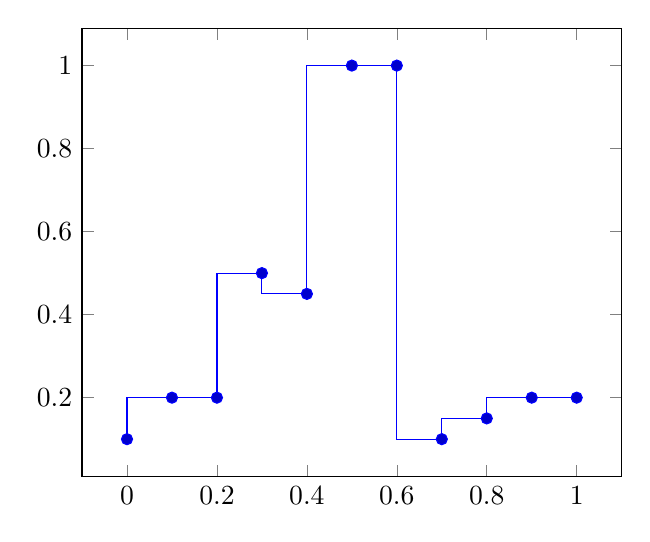
\begin{tikzpicture}
	\begin{axis}
	\addplot+[const plot mark right]
		coordinates {(0,0.1) (0.1,0.2) (0.2,0.2) (0.3,0.5) (0.4,0.45) (0.5,1) (0.6,1) (0.7,0.1) (0.8,0.15) (0.9,0.2) (1,0.2)};
	\end{axis}
\end{tikzpicture}
\end{document}
